% \documentclass[12pt]{article}

%%v helpful MIT exam schema, see http://www-math.mit.edu/~psh/exam/examdoc.pdf
 \documentclass[12pt]{exam} 
% \qformat{\textbf{Question \thequestion}\quad \thepoints\hfill } % Large depth to make space}
 \renewcommand{\thesubpart}{(\roman{subpart})}
 \renewcommand{\subpartlabel}{\thesubpart}
% \footer{}{}{Page \thepage\ de \numpages}
\addpoints
\pointsinmargin
% \boxedpoints
\renewcommand{\questionshook}{\setlength{\itemsep}{4mm}}
\renewcommand{\partshook}{
	\setlength{\itemsep}{0.2cm}
}

\usepackage{cmbright}

\pagestyle{empty} %for handouts
\addtolength{\jot}{2em} % this makes all formulae a bit more spaced vertically for handouts
\setlength{\parindent}{0pt} %we're not writing a novel
\renewcommand{\arraystretch}{1.5} %makes tables taller, so easier to write in

\usepackage[fleqn]{amsmath}
\usepackage{amssymb} %standard classy maths symbols
\usepackage[a4paper, margin=1in]{geometry} %makes it easy to specify where to put stuff on the page

\usepackage{siunitx} %v handy way of getting SI units to typeset correctly...
% \sisetup{locale = FR} %... and now it will use a comma for decimals

\usepackage[utf8]{inputenc}

% \usepackage[french]{babel} % frenchify everything (e.g. a Table becomes a Tableau)
% \usepackage{lmodern} % font with nicer French characters than standard
% \usepackage{textcomp} % and more help for special characters

\usepackage{tcolorbox} % basic but good package for boxes around text
\tcbset{colback=black!5!white}
% \usepackage{color} % colours
%\newcommand{\fillin}{\color{black!1!white}} %makes the text disappear
%\definecolor{fillin}{rgb} {1.00,1.00,1.00}
%\renewcommand{\fillin}{\color{blue}} \definecolor{fillin}{rgb} {0.00,0.00,1.00} %makes the filling in text appear (in blue)

\usepackage{enumitem} % can change the labels on lists, items, enumerates
\usepackage{setspace}

\usepackage{tikz, tkz-euclide} % interval diagrams, sets, etc.
%\usetikzlibrary{calc,trees,positioning,arrows,fit,shapes}

\begin{document}

\textbf{Name:} \dotfill

\
\begin{questions}


\question[2] \textbf{Write down} \emph{(écrire)} the equation for the area of a square of sidelength $a$.

$A(\mbox{square}) = $ \dotfill

Write down the equation for the area of a triangle of base $b$ and height $h$.
\fillwithdottedlines{7mm}

\question[4] Find the \textbf{shaded} \emph{(ombragés)} areas. \emph{State a formula before using it!}

\begin{minipage}{0.7\textwidth}
\fillwithdottedlines{70mm}
\end{minipage}
\begin{minipage}{0.3\textwidth}
\begin{center}

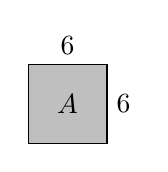
\begin{tikzpicture}
\fill[black!25] (0, 0) rectangle (1,1);
\draw (0, 0) rectangle (1,1) node[pos=.5] {$A$};
\draw (1,0) -- node[right] {6} (1,1) -- node[above] {6} (0,1);
\end{tikzpicture}

\vspace{3mm}

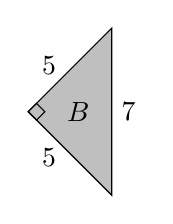
\begin{tikzpicture}[scale=1.5,rotate=-45]
\coordinate (A) at (1,0);
\coordinate (B) at (0,0);
\coordinate (C) at (0,1);

\fill[black!25] (A) --(B) -- (C) -- cycle;
\draw (A) -- (B) -- (C) -- cycle;
\draw (B) rectangle ++(.1,.1);
\node at (-0.15,0.4) {5};
\node at (0.4,-0.15) {5};
\node at (0.3,0.3) {$B$};
\node at (0.6,0.6) {7};
%\draw (1,0) -- node[right] {5} (1,1) -- node[above] {5} (0,1);
\end{tikzpicture}

\vspace{3mm}

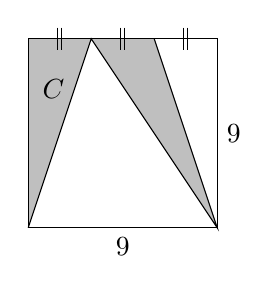
\begin{tikzpicture}[scale=0.8]
\coordinate (O) at (0,0);
\coordinate (A) at (3,0);
\coordinate (B) at (3,3);
\coordinate (C) at (0,3);

\coordinate (S) at (1,3);
\coordinate (T) at (2,3);


\fill[black!25] (O) -- (A) --(B) -- (C) -- cycle;
\fill[white] (O) -- (S) -- (A) -- cycle;
\fill[white] (A) -- (T) -- (B) -- cycle;

\draw (O)-- node[below] {9}  (A) -- node[right] {9} (B) -- (C) -- cycle;
\draw (O) -- (S) --  (A) -- (T);
\tkzMarkSegment[pos=.5,mark=||](C,S) 
\tkzMarkSegment[pos=.5,mark=||](S,T) 
\tkzMarkSegment[pos=.5,mark=||](T,B) 

\node at (0.4, 2.2) {$C$};

%\draw (1,0) -- node[right] {5} (1,1) -- node[above] {5} (0,1);
\end{tikzpicture}


\end{center}
\end{minipage}

\vfill

\question \textbf{Bonus.} 
What fraction of the parallelogram is shaded? 

\hfill \textbf{Work on the back} \emph{(travailler sur le verso.)}

\begin{center}
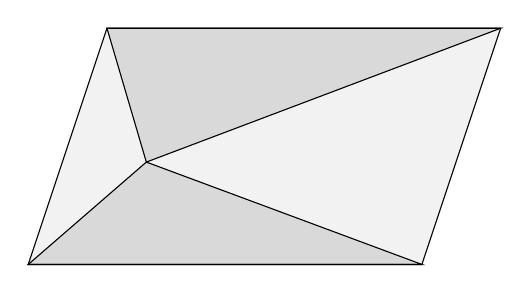
\begin{tikzpicture}

\fill[black!5] (0,0) -- (5,0) -- (6,3) -- (1,3) -- cycle;
\fill[black!15] (0,0) -- (1.5,1.3) -- (5,0) -- cycle;
\fill[black!15] (1,3) -- (1.5,1.3) -- (6,3) -- cycle;
\draw (0,0) -- (5,0) -- (6,3) -- (1,3) -- cycle;
\draw (0,0) -- (1.5,1.3) -- (5,0) -- cycle;
\draw (1,3) -- (1.5,1.3) -- (6,3) -- cycle;


\end{tikzpicture}
\end{center}


\end{questions}

\begin{tcolorbox}

\textbf{Name of the marker:}

\begin{center}
\gradetable[h][questions]
\end{center}

\end{tcolorbox}

\end{document}